\documentclass{article}
\usepackage{amsfonts,graphicx,verbatim}
%%%%%%%%%%%%%%%%%%%%%%%%%%%%%%%%%%%%%%%%%%%%%%%%%%%%%%%%%%%%%%%%
%  6.826 (POCS Seminar) macro file for handouts and problem sets.
%
% You should save this file as handout.tex
%
% Your main LaTeX file should look like this:
%
%        \documentstyle[12pt]{article}
%
%        %%%%%%%%%%%%%%%%%%%%%%%%%%%%%%%%%%%%%%%%%%%%%%%%%%%%%%%%%%%%%%%%
%  6.826 (POCS Seminar) macro file for handouts and problem sets.
%
% You should save this file as handout.tex
%
% Your main LaTeX file should look like this:
%
%        \documentstyle[12pt]{article}
%
%        %%%%%%%%%%%%%%%%%%%%%%%%%%%%%%%%%%%%%%%%%%%%%%%%%%%%%%%%%%%%%%%%
%  6.826 (POCS Seminar) macro file for handouts and problem sets.
%
% You should save this file as handout.tex
%
% Your main LaTeX file should look like this:
%
%        \documentstyle[12pt]{article}
%
%        \input{handout}
%%%%%%%%%%%%%%%%%%%%%%%%%%%%%%%%%%%%%%%%%%%%%%%%%%%%%%%%%%%%%%%%

\oddsidemargin 0in
\evensidemargin 0in
\marginparwidth 40pt
\marginparsep 10pt
\topmargin 0pt
\headsep 0in
\headheight 0in
\textheight 8.5in
\textwidth 6in
\brokenpenalty=10000

% \handout{number}{date}{title}

\newcommand{\handout}[3]{


\begin{center}
\rule{\textwidth}{.0075in} \\
\rule[3mm]{\textwidth}{.0075in}\\

CMU 17-651\hfill Models of Software Systems\hfill Fall 2018\\[3ex]

{\Large\bf #3}\\[3ex]

Dario A Lencina-Talarico \hfill {\bf Handout #1} \hfill #2

\rule{\textwidth}{.0075in} \\
\rule[3mm]{\textwidth}{.0075in} \\
\end{center}

}

% \homework{number}{date}{title}{due-date}
\newcommand{\homework}[4]{

\begin{center}
\rule{\textwidth}{.0075in} \\
\rule[3mm]{\textwidth}{.0075in}\\

CMU 17-651\hfill Models of Software Systems\hfill Fall 2018\\[3ex]

{\Large\bf #3} \\[3ex]

Dario A Lencina Talarico \hfill  #1  \hfill Due: #2\\

\rule{\textwidth}{.0075in} \\
\rule[3mm]{\textwidth}{.0075in} \\
\end{center}

%\noindent
%{\bf Due date: #4}

}

% \solutionset{number}{date}{title}{due-date}
\newcommand{\solutionset}[4]{

\begin{center}
\rule{\textwidth}{.0075in} \\
\rule[3mm]{\textwidth}{.0075in}\\

CMU 17-651\hfill Models of Software Systems\hfill Fall 2016\\[3ex]

{\Large\bf #3} \\[3ex]

Garlan  \hfill  Solutions for Homework #1  \hfill  #2\\

\rule{\textwidth}{.0075in} \\
\rule[3mm]{\textwidth}{.0075in} \\
\end{center}

%\noindent
%{\bf Due date: #4}

}

% \problem{problem-number}
\newcommand{\problem}[1]{
\vspace{2ex}
\noindent
{\bf Problem #1.}

}

% \solution{solution-number}{points}
\newcommand{\solution}[2]{
\vspace{3ex}
\noindent
{\bf Problem #1}  (#2 points)

}

\newcommand{\cscomment}{
\vspace{1ex}
\noindent Comments: }

% \parts{part-alphabet}{points}
\newcommand{\parts}[2]{
\vspace{2ex}
\noindent
{\bf (#1)}  (#2 points)

}

% \problems{problems-number}{points}
\newcommand{\problems}[2]{
\vspace{3ex}
\noindent
{\bf Problem #1}  (#2 points)

}

\newenvironment{symbolfootnotes}{\def\thefootnote{\fnsymbol{footnote}}}{}

%%%%%%%%%%%%%%%%%%%%%%%%%%%%%%%%%%%%%%%%%%%%%%%%%%%%%%%%%%%%%%%%

\oddsidemargin 0in
\evensidemargin 0in
\marginparwidth 40pt
\marginparsep 10pt
\topmargin 0pt
\headsep 0in
\headheight 0in
\textheight 8.5in
\textwidth 6in
\brokenpenalty=10000

% \handout{number}{date}{title}

\newcommand{\handout}[3]{


\begin{center}
\rule{\textwidth}{.0075in} \\
\rule[3mm]{\textwidth}{.0075in}\\

CMU 17-651\hfill Models of Software Systems\hfill Fall 2018\\[3ex]

{\Large\bf #3}\\[3ex]

Dario A Lencina-Talarico \hfill {\bf Handout #1} \hfill #2

\rule{\textwidth}{.0075in} \\
\rule[3mm]{\textwidth}{.0075in} \\
\end{center}

}

% \homework{number}{date}{title}{due-date}
\newcommand{\homework}[4]{

\begin{center}
\rule{\textwidth}{.0075in} \\
\rule[3mm]{\textwidth}{.0075in}\\

CMU 17-651\hfill Models of Software Systems\hfill Fall 2018\\[3ex]

{\Large\bf #3} \\[3ex]

Dario A Lencina Talarico \hfill  #1  \hfill Due: #2\\

\rule{\textwidth}{.0075in} \\
\rule[3mm]{\textwidth}{.0075in} \\
\end{center}

%\noindent
%{\bf Due date: #4}

}

% \solutionset{number}{date}{title}{due-date}
\newcommand{\solutionset}[4]{

\begin{center}
\rule{\textwidth}{.0075in} \\
\rule[3mm]{\textwidth}{.0075in}\\

CMU 17-651\hfill Models of Software Systems\hfill Fall 2016\\[3ex]

{\Large\bf #3} \\[3ex]

Garlan  \hfill  Solutions for Homework #1  \hfill  #2\\

\rule{\textwidth}{.0075in} \\
\rule[3mm]{\textwidth}{.0075in} \\
\end{center}

%\noindent
%{\bf Due date: #4}

}

% \problem{problem-number}
\newcommand{\problem}[1]{
\vspace{2ex}
\noindent
{\bf Problem #1.}

}

% \solution{solution-number}{points}
\newcommand{\solution}[2]{
\vspace{3ex}
\noindent
{\bf Problem #1}  (#2 points)

}

\newcommand{\cscomment}{
\vspace{1ex}
\noindent Comments: }

% \parts{part-alphabet}{points}
\newcommand{\parts}[2]{
\vspace{2ex}
\noindent
{\bf (#1)}  (#2 points)

}

% \problems{problems-number}{points}
\newcommand{\problems}[2]{
\vspace{3ex}
\noindent
{\bf Problem #1}  (#2 points)

}

\newenvironment{symbolfootnotes}{\def\thefootnote{\fnsymbol{footnote}}}{}

%%%%%%%%%%%%%%%%%%%%%%%%%%%%%%%%%%%%%%%%%%%%%%%%%%%%%%%%%%%%%%%%

\oddsidemargin 0in
\evensidemargin 0in
\marginparwidth 40pt
\marginparsep 10pt
\topmargin 0pt
\headsep 0in
\headheight 0in
\textheight 8.5in
\textwidth 6in
\brokenpenalty=10000

% \handout{number}{date}{title}

\newcommand{\handout}[3]{


\begin{center}
\rule{\textwidth}{.0075in} \\
\rule[3mm]{\textwidth}{.0075in}\\

CMU 17-651\hfill Models of Software Systems\hfill Fall 2018\\[3ex]

{\Large\bf #3}\\[3ex]

Dario A Lencina-Talarico \hfill {\bf Handout #1} \hfill #2

\rule{\textwidth}{.0075in} \\
\rule[3mm]{\textwidth}{.0075in} \\
\end{center}

}

% \homework{number}{date}{title}{due-date}
\newcommand{\homework}[4]{

\begin{center}
\rule{\textwidth}{.0075in} \\
\rule[3mm]{\textwidth}{.0075in}\\

CMU 17-651\hfill Models of Software Systems\hfill Fall 2018\\[3ex]

{\Large\bf #3} \\[3ex]

Dario A Lencina Talarico \hfill  #1  \hfill Due: #2\\

\rule{\textwidth}{.0075in} \\
\rule[3mm]{\textwidth}{.0075in} \\
\end{center}

%\noindent
%{\bf Due date: #4}

}

% \solutionset{number}{date}{title}{due-date}
\newcommand{\solutionset}[4]{

\begin{center}
\rule{\textwidth}{.0075in} \\
\rule[3mm]{\textwidth}{.0075in}\\

CMU 17-651\hfill Models of Software Systems\hfill Fall 2016\\[3ex]

{\Large\bf #3} \\[3ex]

Garlan  \hfill  Solutions for Homework #1  \hfill  #2\\

\rule{\textwidth}{.0075in} \\
\rule[3mm]{\textwidth}{.0075in} \\
\end{center}

%\noindent
%{\bf Due date: #4}

}

% \problem{problem-number}
\newcommand{\problem}[1]{
\vspace{2ex}
\noindent
{\bf Problem #1.}

}

% \solution{solution-number}{points}
\newcommand{\solution}[2]{
\vspace{3ex}
\noindent
{\bf Problem #1}  (#2 points)

}

\newcommand{\cscomment}{
\vspace{1ex}
\noindent Comments: }

% \parts{part-alphabet}{points}
\newcommand{\parts}[2]{
\vspace{2ex}
\noindent
{\bf (#1)}  (#2 points)

}

% \problems{problems-number}{points}
\newcommand{\problems}[2]{
\vspace{3ex}
\noindent
{\bf Problem #1}  (#2 points)

}

\newenvironment{symbolfootnotes}{\def\thefootnote{\fnsymbol{footnote}}}{}
\newcommand{\implies}{\Rightarrow}
\newcommand{\until}{\,\mathcal{U}\,}

\begin{document}

\homework{\hspace*{1.15in}Homework \#13}{26 November 2018}{Petri Nets 1}{}



\begin{enumerate}

\item Consider a small garden, similar to the one described by Kramer and Magee, that has two entrances, an East entrance and a West entrance. Users may enter or leave either entrance through a small gate that permits only one user to enter or leave at a time. The park can hold up to 10 people. Model this system using a Petri Net. \\
  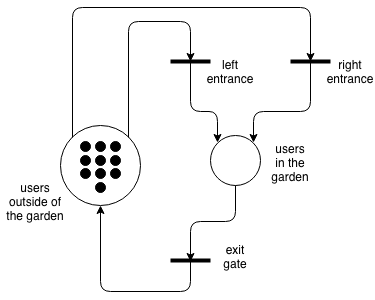
\includegraphics[scale=0.5]{hw13p1.png} \\
  The left entrance and right entrance transitions are not synchronized, users can enter through either entrance. When the users enter, a token is moved from ``users outside the garden'' to ``users in the garden''. \\
  \\
  The diagram resembles the physical setup of the garden which is quite suspicious to me but I believe that the implementation is correct. \\

\item Consider a traffic light that controls traffic on a two-lane road. The light is normally green, allowing cars to pass through. But when a user presses a button, the traffic light should turn yellow, and then red, allowing some number of users to cross the street. It then turns green again, and users are prohibited from crossing.
    \begin{enumerate}
    \item Describe this system using a Petri Net. \\
      I was extremely confused by this question, at the beggining I went down the path of thinking of an ideal system were the traffic light acts as the arbiter for determining who gets to move (vehicles or pedestrians) that would make sense in an ideal world, in reality, both pedestrians and vehicles can be modeled as its own independent subsystems that might colide as they do in real life. \\
      \\
      My implementation proposes that the traffic light subsystem is independent of the rest of the network components and toggles between green - yellow - red without synchronizing with anyone else, like most real semaphores (no v to x technology). \\
      It is the responsability of the pedestrians and vehicles to respect the law and stop/start moving when they receive the traffic light transitions. \\
       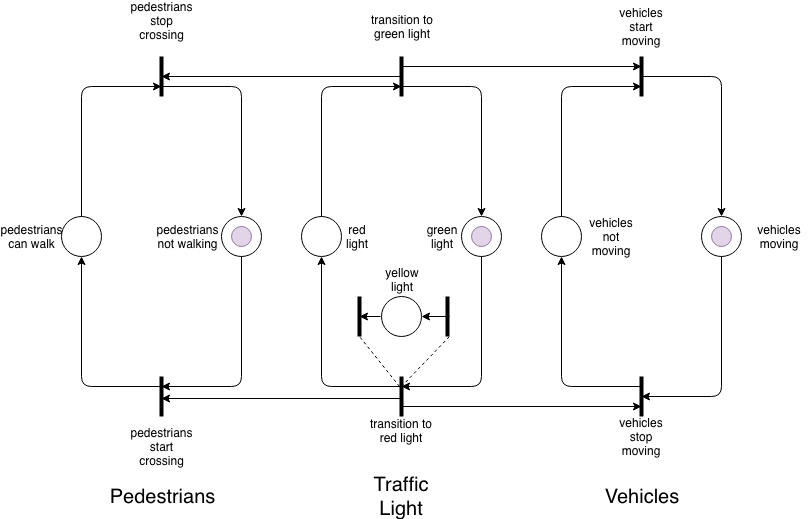
\includegraphics[scale=0.5]{hw13p2.png} \\
     \item Does your net guarantee that the light cannot turn red without first turning yellow? Justify briefly. \\
       Yes, I used the Duration design pattern described in Lecture 23 so that the transition from green to red is ``detailed''.
    It's is labeled in the diagram as ``transition to red light''.
  \item Does your net guarantee that an arriving car will eventually be allowed to pass through the light? \\
    It guarantees that the traffic light will transition to green and signal the vehicles, but pedestrians can be dumb and just block the lanes if they want to.
  \item List three aspects of the real system that are abstracted away by your model. \\
    In my diagram there's no mention of how many vehicles can drive through concurrently, I did not discuss the capacity of the pedestrian crossing or the duration of the traffic light. \\
    \end{enumerate}


\item For the P/V Petri Net shown in Figure 15 of Peterson's article
(Pet77.pdf, page 234):
\\ Ran out of time but will do my best to submit a decent redo with this section.
\begin{enumerate}
 \item  Construct the reachability tree, using the tree condensation
        algorithm shown in class. Assume that the ordering of places in the state vector of the Petri Net shown in Figure 15 is:
(P1, P2, P3, P4, S).


 \item Use this to argue that the design is correct, i.e., that it is
       not possible for the system to be simultaneously in the
       critical sections of both processes.
\end{enumerate}

\end{enumerate}
\end{document}
